% =====================================================================
% Previsão de Produtividade Municipal da Soja no RS com Machine Learning
% Integrantes: Isabelle Franco (RA 10425395), Gustavo Rodrigues (RA 10403091),
%              Pedro Henrique (RA 10388298), Lorenzo Tadeo (RA 10420067)
% Orientador: Prof. Dr. Ivan Carlos Alcântara de Oliveira
% Disciplina: Inteligência Artificial -- Universidade Presbiteriana Mackenzie
%
% Síntese do conteúdo deste arquivo: fonte LaTeX (template SBC) do artigo
% final do projeto (N2), com introdução, fundamentação teórica, metodologia,
% dataset, resultados completos, aspectos éticos, conclusão e referências.
%
% Histórico de alterações:
% Data       | Autor             | Descrição
% -----------|-------------------|------------------------------------------
% 2026-09-24 | Isabelle Franco   | Criação do artigo parcial (N1) no template SBC
% 2026-09-25 | Lorenzo Tadeo     | Figuras 1--3 da análise exploratória (N1)
% 2026-11-19 | Gustavo Rodrigues | Reestruturação para a N2: motivação, contribuições alcançadas, fundamentação teórica e trabalhos relacionados
% 2026-11-19 | Pedro Henrique    | Metodologia completa, adubação fosfatada, arquitetura (Fig. 4) e protocolo de avaliação
% 2026-11-19 | Isabelle Franco   | Resultados completos (Figs. 5--9, Tabs. 4--7), ética e conclusão
% 2026-11-19 | Lorenzo Tadeo     | Revisão geral, referências e endereços do GitHub/YouTube
% =====================================================================
\documentclass[12pt]{article}

\usepackage{sbc-template}
\usepackage{graphicx,url}
\usepackage{amsmath,amssymb}
\usepackage[utf8]{inputenc}
\usepackage[brazil]{babel}
% ATENÇÃO: o template original da SBC carrega \usepackage[latin1]{inputenc}
% logo após a linha acima. Isso gera erro de compilação ("Option clash for
% package inputenc") porque o pacote é carregado duas vezes com opções
% diferentes. Como este arquivo é salvo em UTF-8, mantenha SOMENTE a linha
% [utf8]{inputenc} e NÃO adicione a linha [latin1]{inputenc}.

\sloppy

\title{Previsão de Produtividade da Soja com Machine Learning: Abordagem Orientada por Variáveis Climáticas e Agrícolas}

\author{Isabelle Franco\inst{1}, Gustavo Rodrigues\inst{1}, Pedro Henrique\inst{1},\\
  Lorenzo Tadeo\inst{1}, Ivan Carlos A. de Oliveira\inst{1}}

\address{Faculdade de Computação e Informática (FCI)\\
  Universidade Presbiteriana Mackenzie -- São Paulo -- SP -- Brasil
  \email{\{10425395, 10403091, 10388298, 10420067\}@mackenzista.com.br}
}

\begin{document}

\maketitle

\begin{center}
\footnotesize
Isabelle Franco -- RA: 10425395 -- \texttt{10425395@mackenzista.com.br}\\
Gustavo Rodrigues -- RA: 10403091 -- \texttt{10403091@mackenzista.com.br}\\
Pedro Henrique -- RA: 10388298 -- \texttt{10388298@mackenzista.com.br}\\
Lorenzo Tadeo -- RA: 10420067 -- \texttt{10420067@mackenzista.com.br}\\
Orientador: Prof.\ Dr.\ Ivan Carlos Alcântara de Oliveira
\end{center}

\begin{abstract}
  Soybean yield in Rio Grande do Sul (RS), Brazil, varies sharply from one
  season to the next, mainly because of droughts. We built and evaluated a
  supervised machine learning pipeline that estimates municipal soybean
  yield (kg/ha) from public data: IBGE/SIDRA Table 1612 (497 municipalities,
  2000--2025), the NOAA Oceanic Niño Index (ONI), daily records from 45 INMET
  weather stations and phosphate fertilization recommendations from
  Embrapa/CQFS-RS/SC. Linear (Ridge) Regression, Random Forest and Gradient
  Boosting were compared against three historical baselines with
  walk-forward temporal validation. Hyperparameters were tuned on the
  2010--2015 seasons, and the 2016--2025 seasons were held out for testing.
  With climate observed during the season, the models reduced the mean
  absolute error relative to the best baseline (5-season moving average,
  696 kg/ha) by 12\% (Ridge), 17\% (Random Forest, the model selected on
  validation) and 19\% (Gradient Boosting, 561 kg/ha). With pre-season
  information alone (yield history, fertilization and ONI), no model
  outperformed the baseline. An ablation study and SHAP explanations show
  that the gain comes from the December--February water balance and heat
  indicators. The fertilization attributes, which can only be derived from
  normative recommendations, added no information. The main limitation is
  that the models underestimate how severe unprecedented droughts are (2020,
  2022). Used as a crop-failure alert, the model is conservative: it reaches
  about 0.6 precision at the 80\% threshold, and the threshold can be
  adjusted.

  \noindent\textbf{Keywords:} soybean; crop yield; machine learning;
  explainable AI; temporal validation.
\end{abstract}

\begin{resumo}
  A produtividade da soja no Rio Grande do Sul (RS) varia muito de uma safra
  para outra, sobretudo por causa das secas. Este trabalho construiu e
  avaliou um pipeline de aprendizado de máquina supervisionado que estima a
  produtividade municipal da soja (kg/ha) a partir de dados públicos: a
  Tabela 1612 do IBGE/SIDRA (497 municípios, 2000--2025), o índice ONI da
  NOAA, dados diários de 45 estações do INMET e recomendações de adubação
  fosfatada da Embrapa/CQFS-RS/SC. Regressão Linear (Ridge), Random Forest e
  Gradient Boosting foram comparados com três linhas de base históricas em
  validação temporal \emph{walk-forward}. Os hiperparâmetros foram ajustados
  nas safras de 2010--2015, e as safras de 2016--2025 ficaram reservadas para
  o teste. Com o clima observado durante a safra, os modelos reduziram o erro
  absoluto médio em relação à melhor linha de base (média móvel de 5 safras,
  696 kg/ha) em 12\% (Ridge), 17\% (Random Forest, o modelo selecionado na
  validação) e 19\% (Gradient Boosting, 561 kg/ha). Apenas com informações
  pré-safra (histórico produtivo, adubação e ONI), nenhum modelo superou a
  linha de base. A ablação e as explicações SHAP mostram que o ganho vem do
  balanço hídrico e dos indicadores de calor de dezembro a fevereiro. Os
  atributos de adubação, que só podem ser derivados de recomendações
  normativas, não acrescentaram informação. A principal limitação é que os
  modelos subestimam a intensidade de secas sem precedente (2020, 2022).
  Usado como alerta de quebra de safra, o modelo é conservador: atinge
  precisão de cerca de 0,6 no limiar de 80\%, e o limiar pode ser ajustado.

  \noindent\textbf{Palavras-chave:} soja; produtividade agrícola;
  aprendizado de máquina; IA explicável; validação temporal.
\end{resumo}

% =====================================================================
\section{Introdução}

\subsection{Contextualização}

A soja é uma das principais commodities do agronegócio brasileiro, e o Rio
Grande do Sul é um dos estados mais expressivos nessa cultura. A
produtividade varia significativamente entre municípios e safras,
condicionada pela interação entre regime de chuvas, temperatura, ocorrência
de veranicos, fenômenos climáticos de larga escala (El Niño/La Niña) e
práticas de manejo do solo -- em especial a adubação fosfatada, relevante
para os solos ácidos e historicamente pobres em fósforo do RS
\cite{sbcs2016}. A Pesquisa Agrícola Municipal (PAM) do IBGE, disponibilizada
pela Tabela 1612 do SIDRA \cite{ibge}, oferece uma série histórica municipal
de rendimento, área e produção, o que permite trabalhar com uma amostra
ampla (muitos municípios $\times$ muitas safras) mantendo uma única
granularidade geográfica -- o município -- dentro de um único estado. Entre
2000 e 2025, o rendimento médio dos municípios gaúchos oscilou entre
662~kg/ha (2005) e 3.331~kg/ha (2017), e quatro das seis últimas safras
(2020, 2022, 2023 e 2025) foram afetadas por estiagens
(Figura~\ref{fig:rendimento-safra}).

\subsection{Justificativa}

Modelos de aprendizado de máquina baseados em árvores, como Random Forest e
Gradient Boosting, são adequados a este problema porque capturam relações
não lineares e interações entre clima, histórico produtivo e localização
\cite{jeong2016,vanklompenburg2020}. A estatística oficial do IBGE para uma
safra colhida em abril só é divulgada por volta de setembro do ano
seguinte; uma estimativa municipal produzida logo após a colheita -- ou, idealmente, já na
semeadura -- pode apoiar o planejamento de cooperativas, órgãos de
assistência técnica e defesa civil, sinalizando com granularidade municipal
onde a quebra tende a ser maior. O objetivo não é substituir avaliações
agronômicas locais nem prever o resultado de uma propriedade específica, mas
oferecer um indicador regional, transparente e reprodutível, construído
inteiramente a partir de dados públicos.

\subsection{Motivação}

As estiagens de 2020, 2022 e 2023 reduziram o rendimento dos municípios do
RS, em média, a 64\%, 58\% e 80\% da média das cinco safras anteriores de
cada município, respectivamente, com prejuízos que se propagam para renda rural, crédito,
seguro e arrecadação municipal. A motivação do grupo foi verificar,
com rigor metodológico (sem vazamento de informação futura e com
comparação contra linhas de base honestas), \emph{quanto} da variação de
produtividade pode de fato ser antecipada com dados abertos -- e
\emph{quais} fatores a explicam --, em linha com os Objetivos de
Desenvolvimento Sustentável 2 (Fome Zero e Agricultura Sustentável) e 13
(Ação contra a Mudança Global do Clima).

\subsection{Objetivo}

O objetivo geral é desenvolver e avaliar uma abordagem de aprendizado de
máquina supervisionado capaz de prever a produtividade da soja (kg/ha) por
município do Rio Grande do Sul e por safra, a partir de variáveis
climáticas, do sinal ENOS (ONI) e de atributos de adubação fosfatada,
comparando o desempenho dos modelos contra linhas de base históricas
simples. Os objetivos específicos são:

\begin{itemize}
  \item consolidar uma base analítica integrada em nível município--safra
    (RS, 2000--2025);
  \item construir atributos climáticos por safra a partir do ONI e dos
    dados observados do INMET;
  \item incorporar atributos de adubação fosfatada (MAP, SS, ST, DAP) com
    base em recomendações agronômicas;
  \item treinar e comparar Regressão Linear, Random Forest e Gradient
    Boosting contra linhas de base históricas, sob validação temporal;
  \item aplicar SHAP ao melhor modelo para identificar os fatores mais
    influentes sobre a produtividade.
\end{itemize}

\subsection{Contribuições alcançadas}

\begin{enumerate}
  \item Um \textbf{painel público município--safra} (12.922 pares, 497
    municípios, 2000--2025) integrando IBGE, NOAA, INMET e Embrapa, com
    cobertura climática ampliada de 55,7\% (N1) para 79,2\% dos pares com
    rendimento, graças à seleção da estação \emph{válida} mais próxima.
  \item Um \textbf{protocolo de avaliação sem vazamento} (walk-forward,
    validação 2010--2015 separada do teste 2016--2025, três linhas de base),
    que evidenciou que o ganho dos modelos depende do clima observado na
    safra: com informação pré-safra, nenhum modelo superou a linha de base.
  \item \textbf{Modelos que reduzem o MAE em 12--19\%} frente à melhor linha
    de base no período de teste, que contém as piores secas da série.
  \item Uma \textbf{análise de explicabilidade (SHAP)} que confirma a
    coerência agronômica do modelo (balanço hídrico de dezembro a fevereiro
    como principal fator) e foi usada para \emph{depurá-lo}, eliminando um
    atributo espúrio (\texttt{ano\_safra}).
  \item A \textbf{demonstração empírica} de que atributos de adubação
    derivados de recomendações normativas não acrescentam informação
    preditiva -- um resultado negativo relevante para trabalhos futuros que
    pretendam usar adubação sem dados observados.
  \item Um \textbf{artefato reprodutível} (\texttt{src/prever\_safra.py})
    que gera o ranking municipal de risco de quebra com explicação
    individual das previsões.
\end{enumerate}

\subsection{Evolução em relação à proposta e à N1}

A Tabela~\ref{tab:evolucao} resume o que foi planejado na proposta/N1, o
que foi entregue e as mudanças justificadas.

\begin{table}[ht]
\centering
\caption{Evolução da proposta. Fonte: elaboração própria (2026).}
\label{tab:evolucao}
\footnotesize
\begin{tabular}{|p{3.6cm}|p{4.6cm}|p{5.0cm}|}
\hline
\textbf{Planejado (proposta/N1)} & \textbf{Entregue (N2)} & \textbf{Mudança e justificativa} \\ \hline
Clima da estação mais próxima & Estação \emph{válida} mais próxima (até 100~km) & Estações em pane deixavam 44\% dos pares sem clima. \\ \hline
Precipitação e temperatura médias out--mar & + período crítico dez--fev, balanço P$-$ETo, calor, dias secos, chuva mensal & Literatura agronômica: déficit na floração/enchimento de grãos explica as quebras \cite{farias2007}. \\ \hline
ONI da safra & ONI pré-safra (ASO+SON) e da safra & Permitir um cenário de previsão na semeadura (cenário A). \\ \hline
Adubação por classe de solo & Dose de P$_2$O$_5$ e equivalentes MAP/SS/ST/DAP, hipótese de teor ``Médio'' & Não há dado público observado; o efeito nulo foi medido e reportado. \\ \hline
Duas linhas de base & Três (incluída média móvel de 5 safras) & Comparação mais exigente, que acompanha a tendência tecnológica. \\ \hline
Divisão treino/teste temporal & Walk-forward com validação e teste separados & Evita selecionar hiperparâmetros olhando o teste. \\ \hline
SHAP no melhor modelo & SHAP fora da amostra + diagnóstico de atributo & Usado também para corrigir o modelo (Seção~\ref{sec:shap}). \\ \hline
\end{tabular}
\end{table}

% =====================================================================
\section{Fundamentação Teórica}

\subsection{Conceitos fundamentais}

\textbf{Aprendizado supervisionado e regressão.} Dado um conjunto de pares
$(\mathbf{x}_i, y_i)$, busca-se uma função $f$ que minimize o erro esperado
de $\hat{y}=f(\mathbf{x})$ em dados \emph{não vistos}
\cite{hastie2009}. Aqui $y$ é o rendimento municipal (kg/ha) e
$\mathbf{x}$ reúne histórico produtivo, clima, ONI, localização e adubação.

\textbf{Regressão Linear com regularização (Ridge).} Ajusta
$\hat{y}=\beta_0+\boldsymbol{\beta}^\top\mathbf{x}$ minimizando o erro
quadrático mais a penalidade $\alpha\|\boldsymbol{\beta}\|_2^2$, que
estabiliza os coeficientes quando há atributos colineares
\cite{hoerl1970} -- como as doses de diferentes adubos, que são múltiplos
umas das outras. É a linha de base interpretável do projeto e, por ser
linear, consegue extrapolar tendências, ao contrário das árvores.

\textbf{Random Forest.} Ensemble de árvores de regressão treinadas por
\emph{bagging} (amostras bootstrap) com sorteio de um subconjunto de
atributos em cada divisão; a previsão é a média das árvores, o que reduz a
variância de uma árvore isolada \cite{breiman2001}.

\textbf{Gradient Boosting.} Constrói árvores rasas sequencialmente, cada
uma ajustada ao gradiente da perda (resíduos) do conjunto anterior, com
taxa de aprendizado que controla o passo \cite{friedman2001}. Usou-se a
variante por histogramas do scikit-learn \cite{pedregosa2011}, inspirada no
LightGBM \cite{ke2017}, que trata valores ausentes nativamente.

\textbf{Limitação comum às árvores.} Uma árvore prevê a média dos alvos de
uma folha; portanto, não extrapola além da faixa vista no treino. Isso é
central para entender os erros nas secas sem precedente
(Seção~\ref{sec:resultados}).

\textbf{Validação temporal e vazamento de dados.} Em séries temporais, a
divisão aleatória usa o futuro para prever o passado e superestima o
desempenho \cite{kaufman2012}. A validação \emph{walk-forward} (origem
móvel) treina apenas com períodos anteriores ao previsto e é o padrão para
avaliar previsões fora da amostra \cite{tashman2000}.

\textbf{Métricas.} MAE (erro absoluto médio, em kg/ha, métrica principal
por ser interpretável e robusta), RMSE (penaliza grandes erros), R$^2$
(fração da variância explicada; pode ser negativo quando o modelo é pior que
prever a média do próprio conjunto de teste) e MAPE.

\textbf{IA Explicável (XAI) e SHAP.} SHAP (\emph{SHapley Additive
exPlanations}) decompõe cada previsão em contribuições aditivas dos
atributos, com base nos valores de Shapley da teoria dos jogos
\cite{lundberg2017}; o algoritmo TreeSHAP calcula esses valores de forma
exata e eficiente para ensembles de árvores \cite{lundberg2020}. SHAP mede
\emph{atribuição} no modelo, e não efeito causal: atributos correlacionados
podem dividir o crédito entre si.

\textbf{Balanço hídrico e evapotranspiração.} A demanda hídrica da soja é
máxima da floração ao enchimento de grãos \cite{farias2007}, que no RS
ocorre aproximadamente de dezembro a fevereiro. O balanço climático
simplificado P$-$ETo compara a chuva com a evapotranspiração de referência,
estimada aqui pelo método de Hargreaves-Samani \cite{hargreaves1985}, que
exige apenas temperaturas máxima/mínima e a radiação extraterrestre
calculada pela latitude \cite{allen1998}.

\subsection{Trabalhos relacionados}

Jeong et al.~\cite{jeong2016} mostraram que Random Forest supera a
regressão linear múltipla na previsão de produtividade de trigo, milho e
batata em diferentes regiões do mundo. A revisão sistemática de Van
Klompenburg et al.~\cite{vanklompenburg2020} identificou temperatura,
chuva e tipo de solo como os atributos mais usados e Random Forest e redes
neurais como os algoritmos mais frequentes, apontando a validação
inadequada como fragilidade recorrente. Para o RS, Nóia Júnior et
al.~\cite{noia2020} e Pilau et al.~\cite{pilau2022} relacionam a fase
fria do ENOS (La Niña) a menor rendimento da soja e a maior ocorrência de
eventos extremos. Von Bloh et al.~\cite{vonbloh2023} compararam modelos
de aprendizado de máquina para previsão de produtividade da soja no Brasil
e reforçam a vantagem de modelos baseados em árvores frente a abordagens
lineares quando há relações não lineares entre clima e rendimento.

\begin{table}[ht]
\centering
\caption{Comparação com trabalhos relacionados. Fonte: elaboração própria (2026).}
\label{tab:relacionados}
\footnotesize
\begin{tabular}{|p{2.6cm}|p{2.7cm}|p{4.0cm}|p{3.6cm}|}
\hline
\textbf{Trabalho} & \textbf{Foco} & \textbf{Principal resultado} & \textbf{Diferença deste trabalho} \\ \hline
Jeong et al. (2016) & Várias culturas e regiões & RF supera regressão linear múltipla & Soja no RS, validação temporal explícita \\ \hline
Van Klompenburg et al. (2020) & Revisão sistemática & Clima e solo são os atributos mais usados; RF e redes neurais os algoritmos mais frequentes & Aplica a recomendação de validação sem vazamento \\ \hline
Nóia Júnior et al. (2020); Pilau et al. (2022) & ENOS e soja no RS & La Niña associada a menor rendimento & Testa o ONI como \emph{preditor}: efeito pequeno \\ \hline
Von Bloh et al. (2023) & ML para soja no Brasil & Árvores superam abordagens lineares & Adubação, SHAP, cenário de semeadura e alerta de quebra \\ \hline
\textbf{Este trabalho} & Soja, 440 municípios do RS & Ganho de 12--19\% no MAE só com clima da safra & -- \\ \hline
\end{tabular}
\end{table}

Em relação a esses trabalhos, o projeto se diferencia por (i) incluir e
avaliar explicitamente atributos de adubação fosfatada; (ii) separar um
cenário de previsão na semeadura de um cenário no fim da safra; (iii)
reportar resultados por safra, região e fase do ENOS, e não apenas um
agregado; e (iv) usar SHAP também como ferramenta de depuração. Por outro
lado, não utiliza sensoriamento remoto (por exemplo, NDVI), fonte
frequentemente usada na literatura de previsão de safras
\cite{vanklompenburg2020} -- uma limitação assumida pelo escopo de dados
tabulares públicos.

% =====================================================================
\section{Metodologia}
\label{sec:metodologia}

\subsection{Abordagem e arquitetura da solução}

A pesquisa é aplicada, quantitativa e preditiva, com unidade de análise
município--safra. O problema é tratado como regressão supervisionada em
painel (municípios empilhados), em vez de séries temporais por município,
porque cada município tem no máximo 26 safras -- pouco para ARIMA ou redes
recorrentes -- e novos municípios foram criados por desmembramento no
período. A Figura~\ref{fig:arquitetura} apresenta a arquitetura: quatro
fontes públicas alimentam a etapa de preparação; os modelos e as linhas de
base passam pela validação temporal; o melhor modelo é explicado com SHAP e
encapsulado no artefato de previsão. Todo o código está em Python
(pandas, NumPy, scikit-learn, SHAP e Matplotlib), no módulo
\texttt{src/soja\_pipeline.py} e no notebook
\texttt{notebooks/modelagem\_n2.ipynb}.

\begin{figure}[ht]
\centering
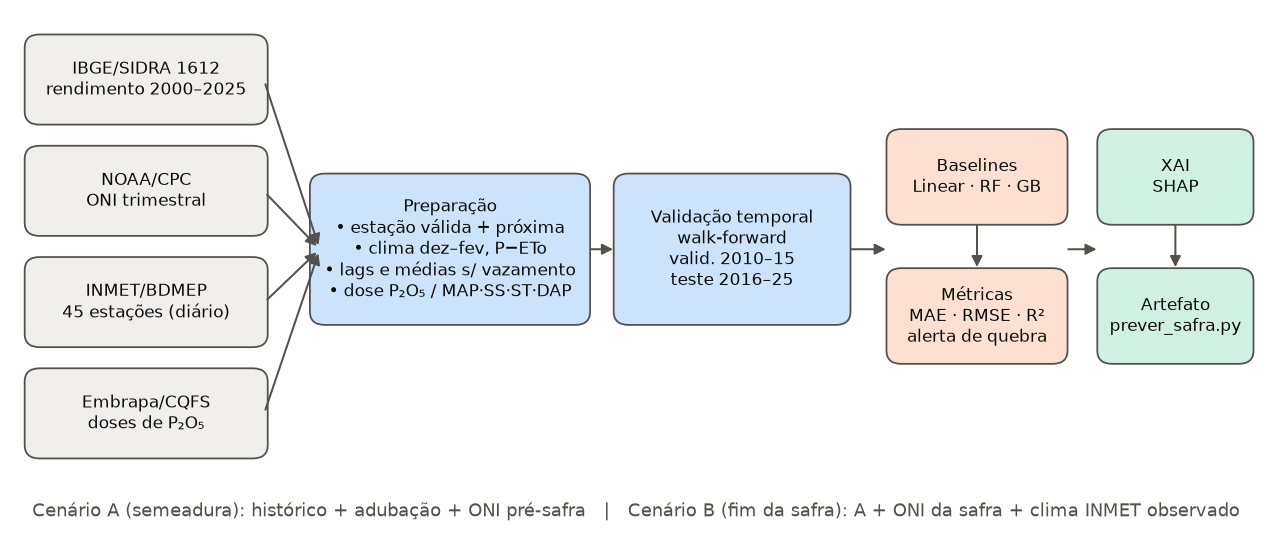
\includegraphics[width=\textwidth]{figuras/fig4_arquitetura.png}
\caption{Arquitetura da solução. Fonte: elaboração própria (2026).}
\label{fig:arquitetura}
\end{figure}

Dois cenários de uso foram definidos conforme a informação disponível no
momento da previsão:
\textbf{Cenário A (semeadura, dezembro):} histórico produtivo, adubação e
ONI pré-safra (16 atributos);
\textbf{Cenário B (fim da safra, abril):} cenário A + ONI da safra + clima
INMET observado (31 atributos). O cenário B antecede em cerca de 17 meses a
divulgação oficial da PAM.

\subsection{Dataset: origem e conteúdo}
\label{sec:origem-bases}

Os dados foram capturados pelo grupo em fontes públicas e oficiais
(Tabela~\ref{tab:fontes}). A descrição detalhada de como cada arquivo foi
obtido está em \texttt{dataset/README.md} no repositório.

\begin{table}[ht]
\centering
\caption{Fontes de dados utilizadas no projeto. Fonte: elaboração própria (2026).}
\label{tab:fontes}
\footnotesize
\begin{tabular}{|p{2.3cm}|p{5.2cm}|p{4.6cm}|}
\hline
\textbf{Fonte} & \textbf{Conteúdo} & \textbf{Uso no projeto} \\ \hline
IBGE/SIDRA -- Tabela 1612 \cite{ibge} & Rendimento (kg/ha), área plantada/colhida e
  produção de soja, 497 municípios do RS, 2000--2025 (API pública). & Variável-alvo e
  histórico produtivo. \\ \hline
NOAA/CPC -- ONI \cite{noaa} & Índice trimestral do ENOS (El Niño/La Niña), 1999--2025. & Sinal
  climático pré-safra e da safra. \\ \hline
INMET / BDMEP \cite{inmet} & Dados diários de 45 estações automáticas do RS (chuva,
  temperaturas), 2000--2025, 280.641 registros. & Clima observado na safra e
  no período crítico. \\ \hline
Embrapa / CQFS-RS/SC \cite{sbcs2016} & Tabelas 2.3 e 2.4: interpretação do teor de P/K e
  doses de P$_2$O$_5$/K$_2$O por classe. & Atributos de adubação
  fosfatada. \\ \hline
\end{tabular}
\end{table}

\subsection{Análise exploratória (N1)}

A análise exploratória (notebook \texttt{analise\_exploratoria.ipynb})
mostrou: (i) cobertura crescente de municípios com soja, de 70,4\% em 2000
para 87,3\% em 2025; (ii) série estadual coerente com eventos conhecidos,
como a seca de 2004/2005 (662~kg/ha, Figura~\ref{fig:rendimento-safra});
(iii) rendimento médio menor sob La Niña ($\approx$2.151~kg/ha) do que em
safras neutras ($\approx$2.432) e de El Niño ($\approx$2.395,
Figura~\ref{fig:rendimento-enos}), compatível com
\cite{noia2020,pilau2022}; e (iv) correlações apenas fracas a moderadas do
rendimento com ONI (0,22) e precipitação out--mar (0,38,
Figura~\ref{fig:correlacao}), indicando que variáveis agregadas simples não
bastam.

\begin{figure}[ht]
\centering
\includegraphics[width=.8\textwidth]{figuras/fig1_rendimento_por_safra.png}
\caption{Rendimento médio da soja nos municípios do RS, por safra
  (2000--2025). Fonte: elaboração própria a partir de IBGE/SIDRA (2026).}
\label{fig:rendimento-safra}
\end{figure}

\begin{figure}[ht]
\centering
\includegraphics[width=.62\textwidth]{figuras/fig2_rendimento_por_enos.png}
\caption{Rendimento médio da soja por fase do ENOS (RS, 2000--2025). Fonte:
  elaboração própria a partir de IBGE/SIDRA e NOAA/CPC (2026).}
\label{fig:rendimento-enos}
\end{figure}

\begin{figure}[ht]
\centering
\includegraphics[width=.68\textwidth]{figuras/fig3_matriz_correlacao.png}
\caption{Matriz de correlação entre as variáveis do painel da N1. Fonte:
  elaboração própria (2026).}
\label{fig:correlacao}
\end{figure}

\subsection{Preparação dos dados}
\label{sec:preparacao}

\textbf{Clima.} Cada dia do INMET é atribuído à safra (out--dez do ano
anterior e jan--mar do ano da safra). Por estação e safra calculam-se:
precipitação e temperatura média out--mar (exigindo $\geq$150 dos
$\sim$182 dias, como na N1) e, no período crítico dez--fev (exigindo
$\geq$75 de 90 dias, com valores normalizados para 90 dias): chuva,
balanço P$-$ETo, Tmax média, dias com Tmax $\geq$32~°C, maior sequência de
dias com chuva $<$1~mm, chuva mensal de novembro a março e anomalia da chuva
em relação à normal da própria estação calculada apenas com safras
anteriores. Cada município recebe o clima da estação \emph{válida} mais
próxima naquela safra (distância de Haversine, até 100~km; mediana de
36,7~km), o que elevou a cobertura climática de 55,7\% para 79,2\% dos
pares com rendimento.

\textbf{Histórico sem vazamento.} Rendimento das safras $t-1$ e $t-2$,
média expandida, média móvel de 5 safras, máximo histórico, número de safras
com registro e logaritmo da área da safra anterior -- todos calculados
exclusivamente com safras anteriores à prevista. Latitude e longitude do
município completam o conjunto.

\textbf{Adubação fosfatada.} Como não existe base pública do fósforo
aplicado por município, adotou-se uma hipótese explícita: solo com teor de
P ``Médio'' em 2º cultivo (Tabela 2.4 da Embrapa/CQFS), com dose-base de
30~kg/ha de P$_2$O$_5$ para 2~t/ha acrescida de 15~kg/ha por tonelada de
rendimento esperado acima de 2~t/ha, sendo o rendimento esperado a média
histórica do município antes da safra. A dose foi convertida em quantidade
equivalente de produto: MAP (52\% de P$_2$O$_5$), Superfosfato Simples
(18\%), Superfosfato Triplo (41\%) e DAP (46\%). A dose média resultante foi
de 32,9~kg/ha de P$_2$O$_5$ (30 a 57), equivalente a 63~kg/ha de MAP ou
183~kg/ha de SS.

\textbf{Base de modelagem.} Mantiveram-se os pares com rendimento
observado, pelo menos 3 safras anteriores com registro e clima válido no
período crítico: 7.951 pares, 440 municípios, safras 2003--2025. Excluir as
safras sem clima (concentradas em 2003--2006, quando poucas estações
operavam) evita que o modelo aprenda, por imputação, que a seca de 2005
ocorreu com clima ``normal''. A Tabela~\ref{tab:dicionario} resume as
principais variáveis.

\begin{table}[ht]
\centering
\caption{Dicionário resumido da base de modelagem. Fonte: elaboração própria (2026).}
\label{tab:dicionario}
\footnotesize
\begin{tabular}{|p{5.0cm}|p{5.6cm}|p{1.5cm}|}
\hline
\textbf{Coluna} & \textbf{Descrição} & \textbf{Unidade} \\ \hline
\texttt{rendimento\_kg\_ha} & Rendimento médio municipal (alvo) & kg/ha \\ \hline
\texttt{rend\_lag1}, \texttt{rend\_media\_5safras} & Rendimento da safra anterior; média das 5 anteriores & kg/ha \\ \hline
\texttt{oni\_pre\_safra}, \texttt{oni\_media\_safra} & ONI médio ASO--SON e OND--JFM & índice \\ \hline
\texttt{balanco\_hidrico\_dez\_fev\_mm} & Chuva menos ETo (Hargreaves) em dez--fev & mm \\ \hline
\texttt{precip\_dez\_fev\_mm}, \texttt{precip\_mar\_mm} & Chuva no período crítico e em março & mm \\ \hline
\texttt{tmax\_dez\_fev\_c}, \texttt{dias\_calor\_dez\_fev} & Tmax média; dias com Tmax $\geq$32~°C & °C / dias \\ \hline
\texttt{dose\_p2o5\_recomendada}, \texttt{kg\_map\_ha\_equiv} (\ldots) & Dose de P$_2$O$_5$ e equivalentes MAP, SS, ST, DAP & kg/ha \\ \hline
\texttt{dist\_estacao\_km} & Distância até a estação usada & km \\ \hline
\end{tabular}
\end{table}

\subsection{Modelos, linhas de base e protocolo de avaliação}

\textbf{Linhas de base:} (i) média histórica expandida do município; (ii)
rendimento da safra anterior; (iii) média móvel das 5 últimas safras.
\textbf{Modelos:} Ridge (com imputação pela mediana, indicadores de
ausência e padronização), Random Forest (300 árvores, imputação e
indicadores de ausência) e Gradient Boosting por histogramas (400
iterações, ausentes tratados nativamente).

\textbf{Walk-forward:} para cada safra $t$, os modelos são treinados com
todas as safras $<t$ e preveem $t$. As safras de \textbf{validação}
(2010--2015) foram usadas para escolher hiperparâmetros por uma grade
pequena (4 configurações por modelo, para não sobreajustar a própria
seleção) e para escolher o modelo principal; as safras de \textbf{teste}
(2016--2025) foram usadas somente para o relatório final. Configurações
escolhidas: Ridge com $\alpha=100$; Random Forest com 5 amostras mínimas
por folha e 60\% dos atributos por divisão; Gradient Boosting com taxa de
aprendizado 0,03 e 31 folhas. Na validação, o Random Forest obteve o menor
MAE (400~kg/ha, contra 406 do Gradient Boosting, 466 da Ridge e 626 da
melhor linha de base) e foi definido como modelo principal.

\textbf{Análises complementares:} erros por safra, fase do ENOS, região
(Norte, Centro e Sul por latitude), porte do município e distância da
estação; uso como \textbf{alerta de quebra} (quebra observada = rendimento
$<$80\% da média histórica; alerta = previsão $<$80\% da média histórica);
\textbf{ablação} por grupo de atributos; e \textbf{SHAP} sobre as previsões
fora da amostra (com o modelo de cada dobra, 120 municípios por safra).

\subsection{Resultados esperados}

Esperava-se que os modelos superassem as linhas de base sobretudo quando as
variáveis climáticas fossem incorporadas e que os resultados indicassem os
limites informacionais dos dados públicos, inclusive se os modelos não
superassem as linhas de base -- o que de fato ocorreu no cenário A.

% =====================================================================
\section{Resultados}
\label{sec:resultados}

\subsection{Aspectos éticos do uso da IA e responsabilidade}

\textbf{Privacidade.} O projeto usa exclusivamente dados públicos agregados
por município ou por estação meteorológica, sem dados pessoais, o que o
mantém aderente à LGPD \cite{lgpd} e dispensa submissão a Comitê de Ética.

\textbf{Vieses e equidade.} Os resultados mostram desempenho desigual: com
o Gradient Boosting, o ganho sobre a linha de base é de 26\% no Norte do
estado (principal região produtora) e de apenas 4\% no Sul, onde a soja é mais recente e as séries
são mais curtas; ali a Ridge chega a ser pior do que a linha de base
(Tabela~\ref{tab:recortes}). Um uso ingênuo do modelo poderia, portanto,
direcionar atenção e recursos às regiões onde ele funciona melhor. Além
disso, municípios pequenos têm na PAM valores frequentemente repetidos
entre safras (estimativas administrativas), o que reduz a qualidade do
alvo. \emph{Mitigação:} publicar o erro por região e por porte junto com
qualquer previsão e não usar o modelo onde o ganho sobre a linha de base
não foi demonstrado.

\textbf{Uso indevido e impacto econômico.} O indicador não deve ser usado
como critério automático de concessão de crédito, precificação de seguro ou
decisão de plantio. Um falso alarme pode prejudicar o acesso a crédito de
um município inteiro; uma quebra não detectada pode atrasar ações de apoio.
Como os dois erros têm custos diferentes, o limiar do alerta deve ser
escolhido por um gestor humano, conforme o contexto
(Seção~\ref{sec:alerta}). \emph{Mitigação:} o artefato apresenta as
previsões como ranking de risco com explicação SHAP, e não como decisão;
recomenda-se manter o humano no ciclo (\emph{human-in-the-loop}) e evitar o
viés de automação.

\textbf{Transparência e responsabilidade.} Código, dados, hiperparâmetros
e resultados estão versionados no GitHub, permitindo auditoria e
reprodução. As limitações estão declaradas: os atributos de adubação são
normativos (não observados) e \emph{não} devem ser lidos como recomendação
de adubação; o modelo subestima secas sem precedente; o SHAP indica
atribuição e não causalidade.

\textbf{Sustentabilidade.} O treinamento completo roda em poucos minutos em
um computador pessoal, com custo energético irrelevante. O uso pretendido
apoia a adaptação às mudanças climáticas (ODS 13) e a segurança alimentar
(ODS 2).

\subsection{Desempenho no teste (2016--2025)}

A Tabela~\ref{tab:metricas} apresenta as métricas agregadas nas 4.158
previsões fora da amostra.

\begin{table}[ht]
\centering
\caption{Métricas no teste walk-forward 2016--2025 (4.158 pares município--safra).
  Ganho = redução do MAE frente à melhor linha de base. Fonte: elaboração própria (2026).}
\label{tab:metricas}
\footnotesize
\setlength{\tabcolsep}{4pt}
\begin{tabular}{|l|l|r|r|r|r|r|}
\hline
\textbf{Cenário} & \textbf{Previsor} & \textbf{MAE} & \textbf{RMSE} & \textbf{R$^2$} & \textbf{MAPE (\%)} & \textbf{Ganho} \\ \hline
-- & Baseline: média histórica & 836,8 & 953,8 & $-$0,18 & 40,3 & $-$20,3\% \\
-- & Baseline: safra anterior & 828,9 & 1.113,5 & $-$0,61 & 48,5 & $-$19,2\% \\
-- & Baseline: média 5 safras & 695,7 & 895,5 & $-$0,04 & 43,3 & -- \\ \hline
A (semeadura) & Regressão Linear (Ridge) & 728,6 & 965,3 & $-$0,21 & 48,1 & $-$4,7\% \\
A (semeadura) & Random Forest & 789,5 & 1.019,0 & $-$0,35 & 46,5 & $-$13,5\% \\
A (semeadura) & Gradient Boosting & 782,0 & 997,5 & $-$0,30 & 44,5 & $-$12,4\% \\ \hline
B (fim da safra) & Regressão Linear (Ridge) & 611,6 & 783,8 & 0,20 & 37,0 & 12,1\% \\
B (fim da safra) & \textbf{Random Forest} (selecionado) & \textbf{576,0} & 760,6 & 0,25 & 34,9 & \textbf{17,2\%} \\
B (fim da safra) & Gradient Boosting & \textbf{560,7} & 745,5 & 0,28 & 33,9 & \textbf{19,4\%} \\ \hline
\end{tabular}
\end{table}

No \textbf{cenário B}, os três modelos superam as três linhas de base em
todas as métricas. O Gradient Boosting obteve o menor erro no teste, embora
o Random Forest tenha sido o escolhido na validação; a diferença entre eles
(15~kg/ha) é pequena diante da variação entre safras e não altera as
conclusões. No \textbf{cenário A}, nenhum modelo supera a média de 5
safras: com o histórico, a adubação normativa e o ONI pré-safra, não foi
possível antecipar as quebras do período de teste. O R$^2$ moderado
(0,25--0,28) reflete que a maior parte da variância no teste vem de choques
que atingem o estado inteiro em poucas safras de seca.

A Figura~\ref{fig:mae-safra} detalha o erro por safra. Os modelos de árvores
vencem a média de 5 safras em 7 das 10 safras de teste, com ganhos maiores
em 2022 (885--993 contra 1.436~kg/ha) e 2024. As exceções são 2020, primeira
grande seca do período de teste, em que todos os previsores erram acima de
1.000~kg/ha; 2021, recuperação recorde em que a Ridge (380~kg/ha) supera as
árvores por conseguir extrapolar a tendência; e 2025.

\begin{figure}[ht]
\centering
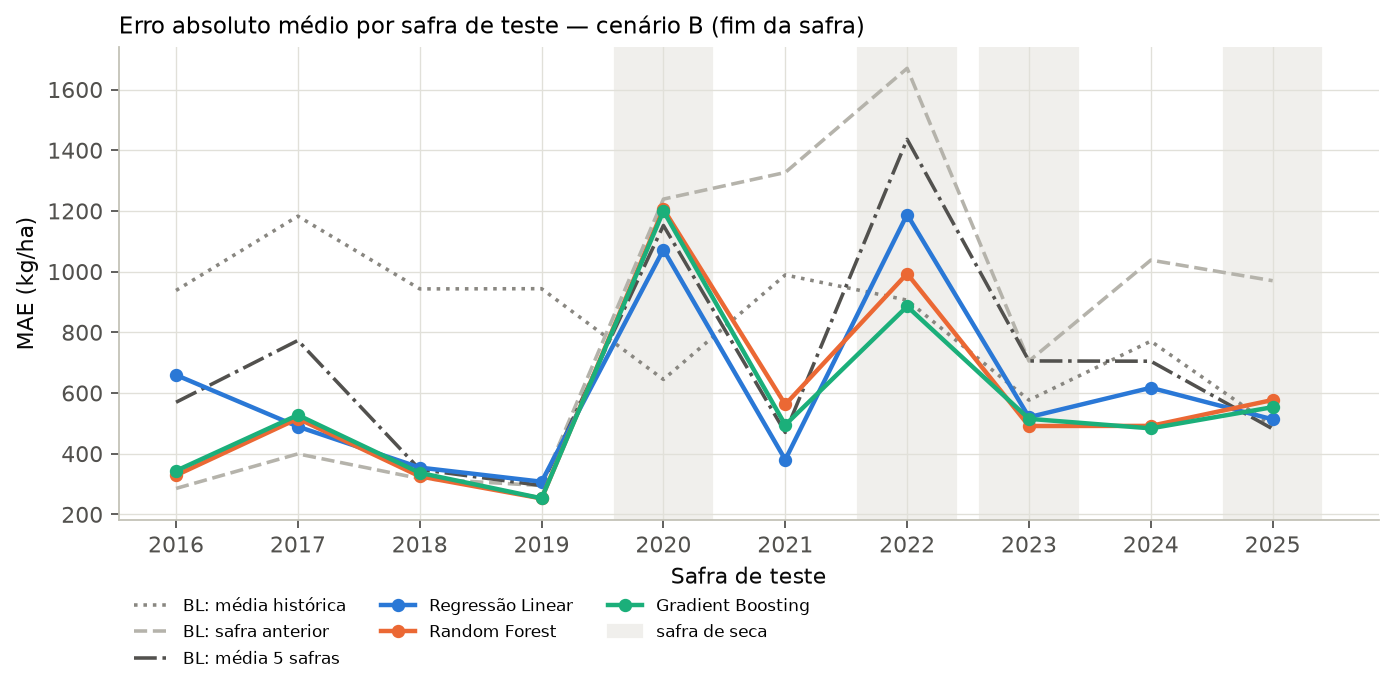
\includegraphics[width=.95\textwidth]{figuras/fig5_mae_por_safra.png}
\caption{MAE por safra de teste, cenário B. Faixas cinzas indicam safras de
  seca. Fonte: elaboração própria (2026).}
\label{fig:mae-safra}
\end{figure}

A Figura~\ref{fig:obs-prev} compara observado e previsto. O modelo
aproxima a nuvem da diagonal, mas há uma faixa de previsões entre 2.000 e
3.500~kg/ha para pares que renderam menos de 1.500~kg/ha: o modelo detecta
a direção da quebra, mas \textbf{subestima sua magnitude} (regressão à
média). Em 2022, a Tmax média de dezembro a fevereiro (31,8~°C) superou a de
todas as safras anteriores (máximo de $\approx$30,5~°C), situação em que
árvores não extrapolam.

\begin{figure}[ht]
\centering
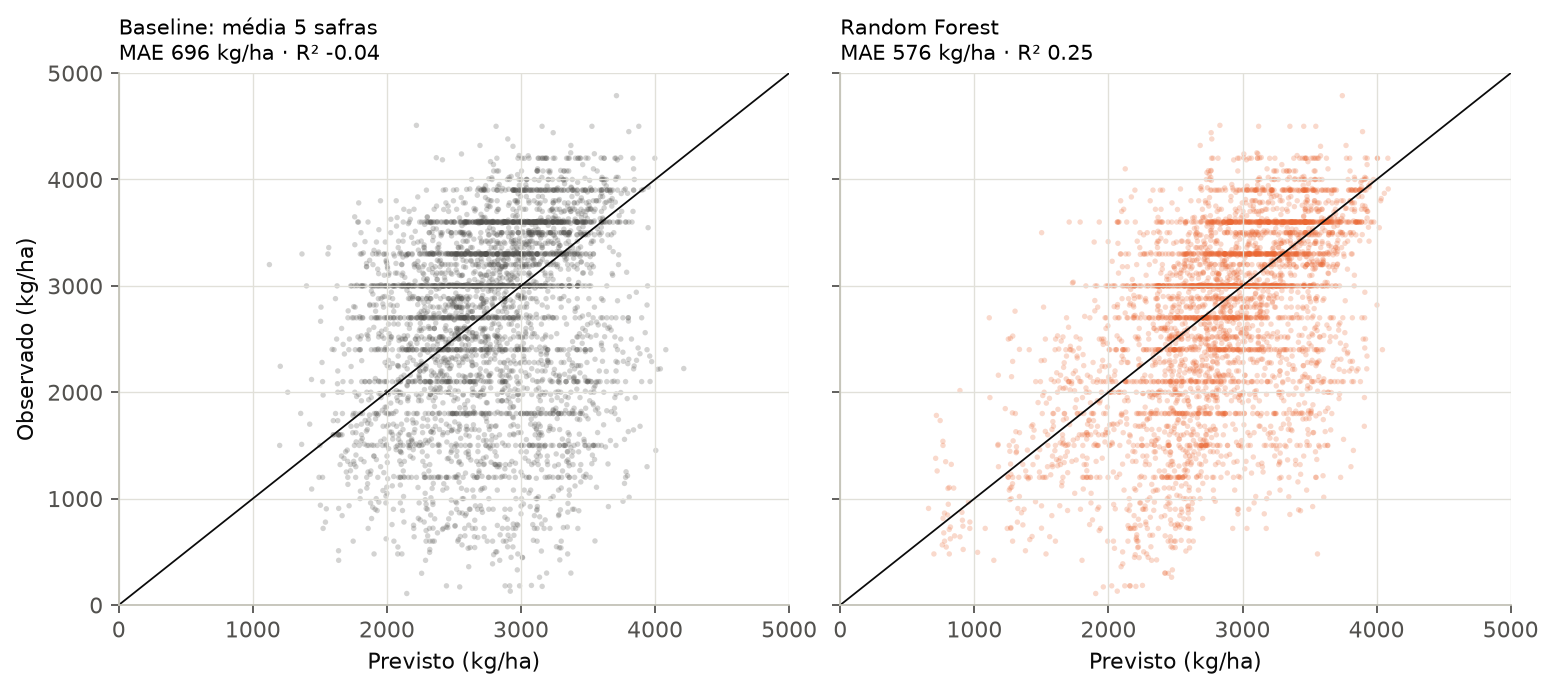
\includegraphics[width=.95\textwidth]{figuras/fig6_observado_previsto.png}
\caption{Observado $\times$ previsto no teste 2016--2025 (cenário B): melhor
  linha de base e Random Forest. Fonte: elaboração própria (2026).}
\label{fig:obs-prev}
\end{figure}

\subsection{Análise de erros por recorte}

\begin{table}[ht]
\centering
\caption{MAE (kg/ha) por recorte no teste, cenário B. Fonte: elaboração própria (2026).}
\label{tab:recortes}
\footnotesize
\begin{tabular}{|l|l|r|r|r|r|r|}
\hline
\textbf{Recorte} & \textbf{Grupo} & \textbf{n} & \textbf{BL 5 safras} & \textbf{Ridge} & \textbf{RF} & \textbf{GB} \\ \hline
Fase ENOS & La Niña & 1.674 & 743 & 613 & 594 & 559 \\
 & Neutro & 823 & 626 & 501 & 546 & 540 \\
 & El Niño & 1.661 & 682 & 665 & 572 & 572 \\ \hline
Região & Norte & 2.301 & 748 & 625 & 577 & 555 \\
 & Centro & 1.478 & 633 & 580 & 567 & 559 \\
 & Sul & 379 & 624 & 655 & 604 & 599 \\ \hline
Distância & $\leq$20 km & 837 & 687 & 614 & 586 & 575 \\
da estação & 20--40 km & 1.797 & 710 & 607 & 571 & 552 \\
 & 40--100 km & 1.524 & 684 & 616 & 576 & 564 \\ \hline
Porte & pequeno & 1.394 & 618 & 571 & 542 & 538 \\
(área) & médio & 1.379 & 708 & 628 & 582 & 563 \\
 & grande & 1.385 & 761 & 605 & 605 & 582 \\ \hline
\end{tabular}
\end{table}

A Tabela~\ref{tab:recortes} mostra que o maior ganho ocorre nas safras de
La Niña (de 743 para 559~kg/ha com o Gradient Boosting), justamente as mais
arriscadas, e no Norte do estado. A distância até a estação não degradou o
desempenho de forma perceptível, o que indica que, até 100~km, a seleção da
estação válida mais próxima é adequada. O mapa da
Figura~\ref{fig:erro-espacial} mostra que os maiores erros se concentram no
centro-norte (Planalto e Depressão Central), onde as quebras de 2020 e 2022
foram mais intensas.

\begin{figure}[ht]
\centering
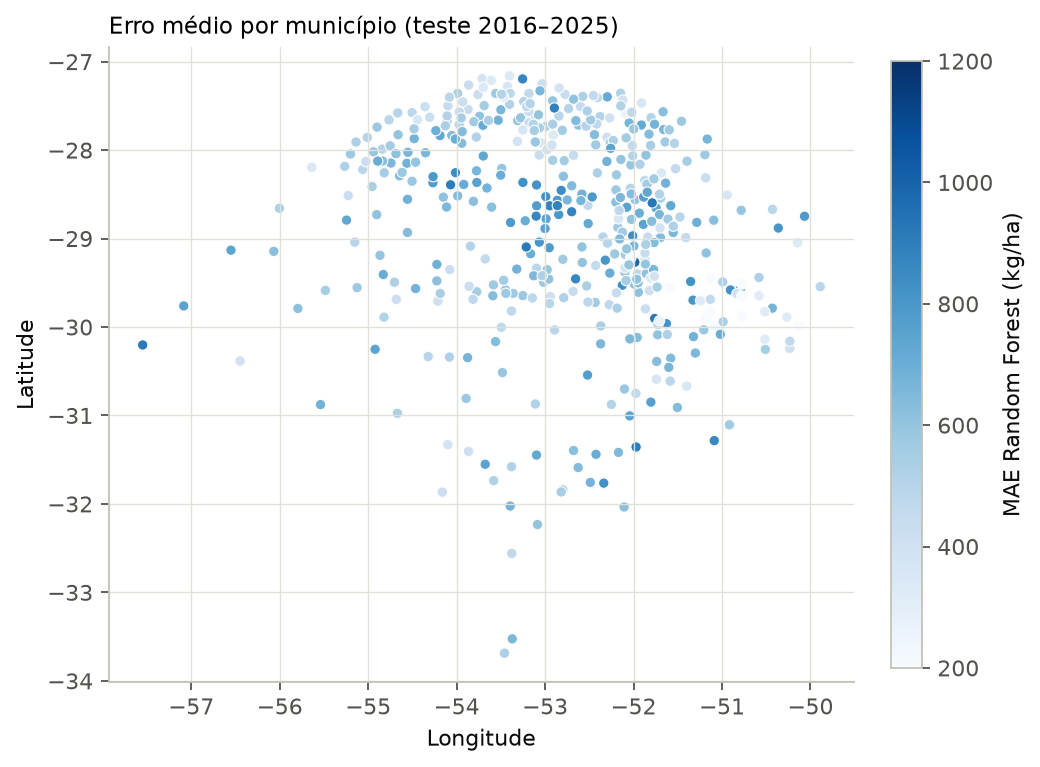
\includegraphics[width=.6\textwidth]{figuras/fig9_erro_espacial.png}
\caption{MAE do Random Forest por município (teste 2016--2025). Fonte:
  elaboração própria (2026).}
\label{fig:erro-espacial}
\end{figure}

\subsection{Uso como alerta de quebra de safra}
\label{sec:alerta}

No teste, 19,6\% dos pares tiveram quebra (rendimento $<$80\% da média
histórica). Com o limiar de 80\%, o Random Forest emitiu 228 alertas, dos
quais 142 se confirmaram (\textbf{precisão 0,62}), mas detectou só 17\% das
quebras (revocação 0,17; F1 0,27). A melhor linha de base quase nunca
alerta (revocação 0,01), e a safra anterior gera muitos falsos alarmes
(precisão 0,22). Elevando o limiar do alerta para 105\% da média histórica,
a revocação sobe para 0,45 com precisão 0,46 (F1 0,45). O modelo é,
portanto, um sinal de risco conservador, cujo limiar deve ser escolhido
pelo usuário conforme o custo relativo de falsos alarmes e de quebras não
detectadas.

\subsection{Ablação: contribuição de cada grupo de atributos}

\begin{figure}[ht]
\centering
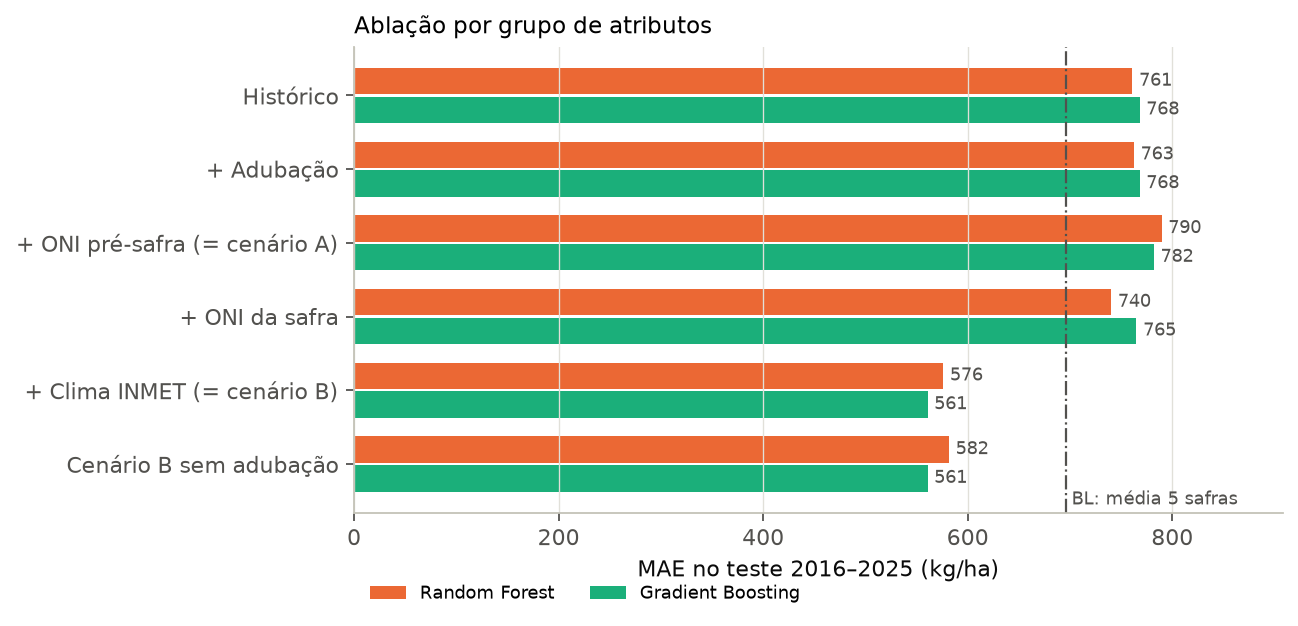
\includegraphics[width=.85\textwidth]{figuras/fig8_ablacao.png}
\caption{MAE no teste conforme os grupos de atributos são adicionados. A
  linha tracejada é a média de 5 safras. Fonte: elaboração própria (2026).}
\label{fig:ablacao}
\end{figure}

A Figura~\ref{fig:ablacao} mostra que somente o histórico leva os modelos
de árvores a um MAE de 761--768~kg/ha, \emph{pior} que a média de 5 safras,
porque elas não extrapolam a tendência de alta da produtividade. Adicionar
adubação não altera o erro (763/768), e o ONI pouco contribui (740--790).
O salto ocorre com o \textbf{clima INMET} (576/561), responsável por todo o
ganho sobre a linha de base. Retirar a adubação do cenário B mantém o erro
(582/561). O resultado era esperado por construção: com classe de solo
única, a dose é uma função monótona da média histórica (correlação de
Spearman de 0,94), e transformações monótonas não acrescentam informação a
árvores de decisão. Trata-se de uma limitação dos dados públicos
disponíveis, e não do método.

\subsection{Explicabilidade com SHAP}
\label{sec:shap}

\begin{figure}[ht]
\centering
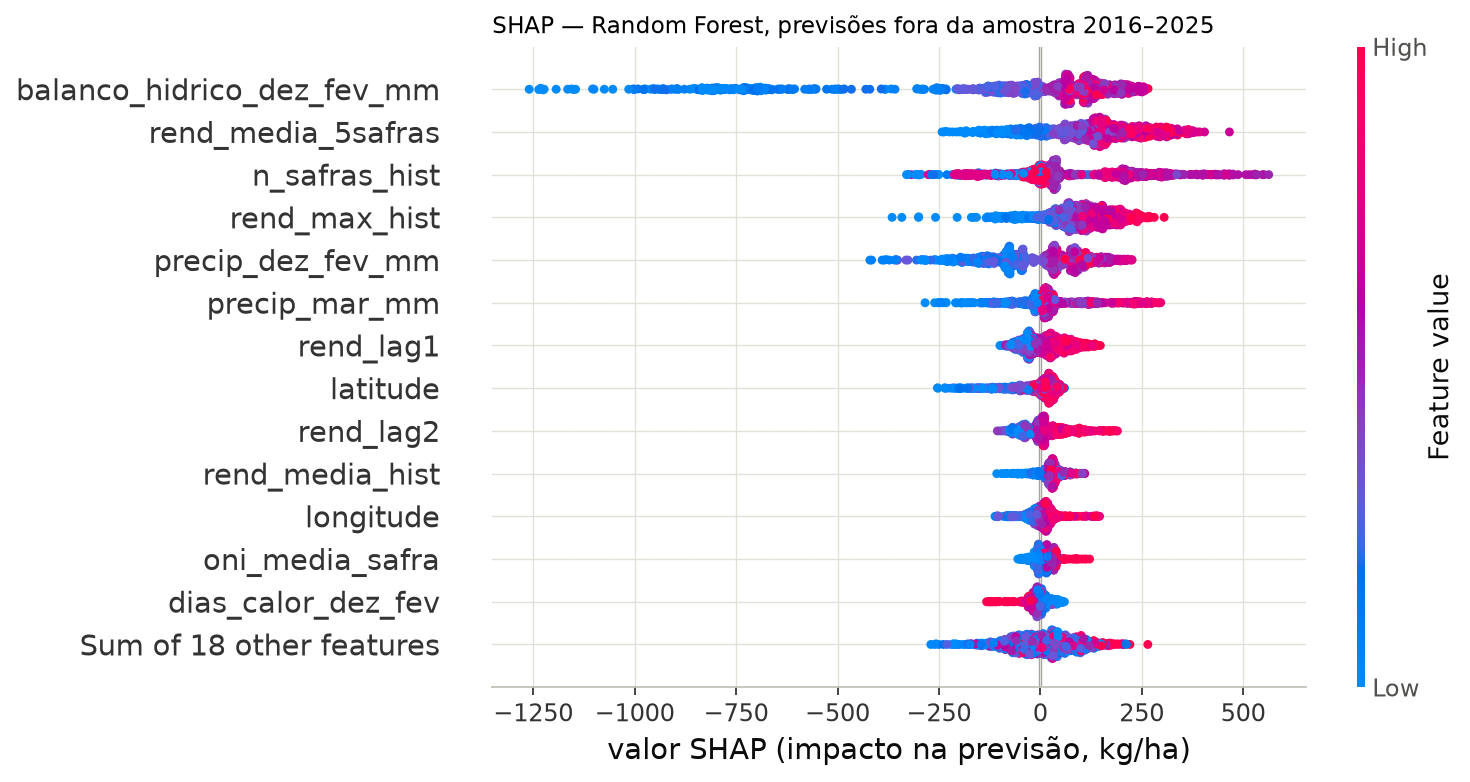
\includegraphics[width=.95\textwidth]{figuras/fig7_shap_resumo.png}
\caption{Valores SHAP do Random Forest nas previsões fora da amostra
  (2016--2025). Cada ponto é um município--safra; a cor indica o valor do
  atributo. Fonte: elaboração própria (2026).}
\label{fig:shap}
\end{figure}

A Figura~\ref{fig:shap} mostra que o \textbf{balanço hídrico de dezembro a
fevereiro} é o atributo mais influente: valores muito negativos (déficit)
reduzem a previsão em até $\sim$1.200~kg/ha. Seguem a média de 5 safras e o
máximo histórico, que definem o patamar do município, a chuva de dez--fev e
de março, e os dias de calor, cujos valores altos reduzem a previsão. Por
grupo, o histórico produtivo concentra 49,9\% da importância média
absoluta, o clima INMET 43,1\%, a adubação 4,5\% e o ONI 2,5\%. Os 4,5\%
atribuídos à adubação, apesar do efeito nulo na ablação, ilustram que o
SHAP divide crédito entre atributos colineares e não mede causalidade.

\textbf{SHAP como ferramenta de depuração.} Na primeira versão do modelo, o
SHAP mostrou o atributo \texttt{ano\_safra} entre os mais importantes, com
safras recentes reduzindo a previsão. Como árvores não extrapolam no tempo,
a safra prevista caía sempre na ``última folha'' do treino e herdava o
regime das safras mais recentes; após a seca de 2020, por exemplo, a
previsão de 2021 era puxada para baixo. O atributo foi removido com base na
\emph{validação} (MAE de 482 para 466 na Ridge, de 413 para 400 no Random
Forest e inalterado em 406 no Gradient Boosting), o que também melhorou o
teste.

\textbf{Explicação local e artefato.} O script
\texttt{src/prever\_safra.py} treina o modelo com as safras anteriores à
safra alvo e gera, por município, a previsão, a referência histórica, o
desvio percentual, o alerta e, opcionalmente, os principais fatores SHAP.
Para Cruz Alta na safra 2022, por exemplo, o balanço hídrico de
$-$406~mm contribuiu com $-$822~kg/ha para a previsão. Na safra 2025, o
artefato emitiu 41 alertas entre 414 municípios, dos quais 27 (66\%) tiveram
quebra confirmada pelo IBGE.

\subsection{Endereços do projeto}

\noindent\textbf{GitHub (artigo, dataset, notebooks, código e resultados):}\\
\url{https://github.com/isah5/Projeto_Safra_de_Soja}

\noindent\textbf{Vídeo de apresentação (YouTube):}\\
\url{https://youtu.be/INSERIR-LINK-DO-VIDEO}

% =====================================================================
\section{Conclusão}

Este trabalho propôs e avaliou uma solução de aprendizado de máquina para
estimar a produtividade municipal da soja no Rio Grande do Sul a partir de
dados públicos. O objetivo geral foi alcançado: foi construída uma base
integrada município--safra, foram treinados e comparados Regressão Linear,
Random Forest e Gradient Boosting contra três linhas de base sob validação
temporal sem vazamento, e o melhor modelo foi explicado com SHAP. Com o
clima observado na safra (cenário B), os modelos reduziram o erro absoluto
médio em 12 a 19\% em relação à melhor linha de base, num período de teste
que inclui as piores secas da série, e o ganho foi maior justamente nas
safras de La Niña e na principal região produtora.

O trabalho também mostrou o que \emph{não} foi possível obter. Na semeadura
(cenário A), o histórico, o ONI e a adubação não bastaram para superar a
média das 5 últimas safras. Os atributos de adubação fosfatada, objetivo
específico da proposta, foram integrados, mas, por serem derivados de
recomendações normativas e não de dados observados, não acrescentaram
informação, o que foi demonstrado pela ablação. Além disso, os modelos
subestimam a magnitude de secas sem precedente, por limitação estrutural de
extrapolação dos modelos de árvores e pelo pequeno número de safras de seca
no treino. Essas conclusões estão sustentadas por evidências reproduzíveis
publicadas no repositório.

Como trabalhos futuros, propõem-se: incorporar índices de vegetação por
satélite (NDVI) e previsões sazonais de chuva para viabilizar o cenário de
semeadura; usar dados observados de fertilidade do solo, como laudos
laboratoriais agregados por município, no lugar da hipótese normativa;
testar alvos relativos (anomalia de rendimento) e modelos com restrições
monotônicas ou componentes lineares, para melhorar a extrapolação em secas
extremas; e calibrar o limiar do alerta junto a usuários reais, como
cooperativas e órgãos de extensão rural.

% =====================================================================
\section*{Referências}

\begin{thebibliography}{99}

\bibitem{allen1998}
ALLEN, R. G.; PEREIRA, L. S.; RAES, D.; SMITH, M. \emph{Crop
evapotranspiration: guidelines for computing crop water requirements}. FAO
Irrigation and Drainage Paper 56. Roma: FAO, 1998.

\bibitem{lgpd}
BRASIL. Lei n.º 13.709, de 14 de agosto de 2018. Lei Geral de Proteção de
Dados Pessoais (LGPD). \emph{Diário Oficial da União}, Brasília, DF, 15 ago.
2018.

\bibitem{breiman2001}
BREIMAN, L. Random forests. \emph{Machine Learning}, v. 45, p. 5--32, 2001.

\bibitem{farias2007}
FARIAS, J. R. B.; NEPOMUCENO, A. L.; NEUMAIER, N. \emph{Ecofisiologia da
soja}. Circular Técnica 48. Londrina: Embrapa Soja, 2007.

\bibitem{friedman2001}
FRIEDMAN, J. H. Greedy function approximation: a gradient boosting machine.
\emph{The Annals of Statistics}, v. 29, n. 5, p. 1189--1232, 2001.

\bibitem{hargreaves1985}
HARGREAVES, G. H.; SAMANI, Z. A. Reference crop evapotranspiration from
temperature. \emph{Applied Engineering in Agriculture}, v. 1, n. 2, p.
96--99, 1985.

\bibitem{hastie2009}
HASTIE, T.; TIBSHIRANI, R.; FRIEDMAN, J. \emph{The elements of statistical
learning}. 2. ed. New York: Springer, 2009.

\bibitem{hoerl1970}
HOERL, A. E.; KENNARD, R. W. Ridge regression: biased estimation for
nonorthogonal problems. \emph{Technometrics}, v. 12, n. 1, p. 55--67, 1970.

\bibitem{ibge}
IBGE -- INSTITUTO BRASILEIRO DE GEOGRAFIA E ESTATÍSTICA. Produção Agrícola
Municipal: tabela 1612 -- lavouras temporárias. Rio de Janeiro: IBGE/SIDRA.
Disponível em: \url{https://sidra.ibge.gov.br/tabela/1612}. Acesso em: 25
set. 2026.

\bibitem{inmet}
INMET -- INSTITUTO NACIONAL DE METEOROLOGIA. BDMEP -- Banco de Dados
Meteorológicos. Brasília, DF. Disponível em:
\url{https://bdmep.inmet.gov.br/}. Acesso em: 25 set. 2026.

\bibitem{jeong2016}
JEONG, J. H. et al. Random forests for global and regional crop yield
predictions. \emph{PLOS ONE}, v. 11, n. 6, e0156571, 2016.

\bibitem{kaufman2012}
KAUFMAN, S.; ROSSET, S.; PERLICH, C.; STITELMAN, O. Leakage in data mining:
formulation, detection, and avoidance. \emph{ACM Transactions on Knowledge
Discovery from Data}, v. 6, n. 4, art. 15, 2012.

\bibitem{ke2017}
KE, G. et al. LightGBM: a highly efficient gradient boosting decision tree.
In: \emph{Advances in Neural Information Processing Systems 30 (NIPS
2017)}. 2017. p. 3146--3154.

\bibitem{lundberg2017}
LUNDBERG, S. M.; LEE, S.-I. A unified approach to interpreting model
predictions. In: \emph{Advances in Neural Information Processing Systems 30
(NIPS 2017)}. 2017. p. 4765--4774.

\bibitem{lundberg2020}
LUNDBERG, S. M. et al. From local explanations to global understanding with
explainable AI for trees. \emph{Nature Machine Intelligence}, v. 2, p.
56--67, 2020.

\bibitem{noaa}
NOAA -- NATIONAL OCEANIC AND ATMOSPHERIC ADMINISTRATION. Climate Prediction
Center. Oceanic Niño Index (ONI): Cold \& Warm Episodes by Season.
Disponível em:
\url{https://origin.cpc.ncep.noaa.gov/products/analysis_monitoring/ensostuff/ONI_v5.php}.
Acesso em: 25 set. 2026.

\bibitem{noia2020}
NÓIA JÚNIOR, R. S. et al. Effects of the El Niño Southern Oscillation
phenomenon and sowing dates on soybean yield and on the occurrence of
extreme weather events in southern Brazil. \emph{Agricultural and Forest
Meteorology}, v. 290, 108038, 2020.

\bibitem{pedregosa2011}
PEDREGOSA, F. et al. Scikit-learn: machine learning in Python. \emph{Journal
of Machine Learning Research}, v. 12, p. 2825--2830, 2011.

\bibitem{pilau2022}
PILAU, F. G. et al. Impact of ENSO-related rainfall variability on soybean
yield in the state of Rio Grande do Sul, Brazil. \emph{Agrometeoros}, v. 30,
e027115, 2022.

\bibitem{sbcs2016}
SOCIEDADE BRASILEIRA DE CIÊNCIA DO SOLO -- NÚCLEO REGIONAL SUL / COMISSÃO
DE QUÍMICA E FERTILIDADE DO SOLO -- RS/SC. \emph{Manual de calagem e
adubação para os Estados do Rio Grande do Sul e de Santa Catarina}. Porto
Alegre, 2016.

\bibitem{tashman2000}
TASHMAN, L. J. Out-of-sample tests of forecasting accuracy: an analysis and
review. \emph{International Journal of Forecasting}, v. 16, n. 4, p.
437--450, 2000.

\bibitem{vanklompenburg2020}
VAN KLOMPENBURG, T.; KASSAHUN, A.; CATAL, C. Crop yield prediction using
machine learning: a systematic literature review. \emph{Computers and
Electronics in Agriculture}, v. 177, 105709, 2020.

\bibitem{vonbloh2023}
VON BLOH, M. et al. Machine learning for soybean yield forecasting in
Brazil. \emph{Agricultural and Forest Meteorology}, v. 341, 109670, 2023.

\end{thebibliography}

\end{document}
